
\begin{figure}[H]
  \centering
  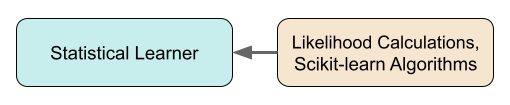
\includegraphics[width=0.7\linewidth]{./chapters/exp1/methodology3.png}
  \caption{Third portion of the flowchart from Figure \ref{fig:method} being 
           described in this section.}
\end{figure}

The chosen algorithms (\textit{k}-nearest neighbors, decision trees, and
\gls{MLL} calculations) are introduced in Section \ref{sec:algs} and their
implementation details are in Section \ref{sec:statmodel1}.  This section will
therefore only cover the implementation differences from the previous work.
The \gls{MLL} calculations are implemented identically to Chapter
\ref{ch:exp1}.  However, the scikit-learn algorithms in this experiment did
undergo a new round of hyperparameter optimization.

The full list of training sets that undergo training and prediction are as
follows: 29 nuclide masses (from Chapter \ref{ch:exp1}), 32 nuclide activities
(full knowledge), 7 \& 12 nuclide activities (full knowledge for short and long
energy window lists, respectively), and auto, short, and long energy window
lists applied to the six detectors (lab-based \gls{HPGe}, portable \gls{HPGe},
\gls{CZT}, \gls{SrI2}, \gls{LaBr3}, \gls{NaI}). Each of these 22 training sets
\todo{left off here} 

Table \ref{tbl:exp2hypparam} lists the updates to the hyperparameter
optimization results. Because the 29 nuclide mass training set is included for
comparison 

\begin{table}[!htb]
  \centering
  \begin{tabular}{@{}llcll@{}}
    \toprule
    \textbf{\begin{tabular}[c]{@{}l@{}}Training Set\\ Description\end{tabular}} &
    \textbf{\begin{tabular}[c]{@{}l@{}}Prediction\\ Parameter\end{tabular}} &
    \textbf{\begin{tabular}[c]{@{}l@{}}\textit{k} \\ (N neighbors)\end{tabular}} &
    \textbf{\begin{tabular}[c]{@{}l@{}}Max \\ Depth\end{tabular}} &
    \textbf{\begin{tabular}[c]{@{}l@{}}Max \\ Features\end{tabular}} \\ 
    \toprule
    \multirow{4}{*}{\begin{tabular}[c]{@{}l@{}}29 \\ Nuclide\\ Masses\end{tabular}}          & Reactor Type & 4 & 56 & 29          \\
                                                                                             & Burnup       & 1 & 77 & 29          \\
                                                                                             & Enrichment   & 1 & 73 & 29          \\
                                                                                             & Cooling Time & 2 & 45 & 29          \\ 
                                                                                             \hline
    \multirow{4}{*}{\begin{tabular}[c]{@{}l@{}}32\\ Nuclide\\ Activities\end{tabular}}       & Reactor Type & 1 & 41 & 32          \\
                                                                                             & Burnup       & 1 & 49 & 32          \\
                                                                                             & Enrichment   & 1 & 67 & 32          \\
                                                                                             & Cooling Time & 7 & 56 & 32          \\
                                                                                             \hline
    \multirow{4}{*}{\begin{tabular}[c]{@{}l@{}}7 or 12\\ Nuclide \\ Activities\end{tabular}} & Reactor Type & 1 & 67 & 7 or 12     \\
                                                                                             & Burnup       & 1 & 78 & 7 or 12     \\
                                                                                             & Enrichment   & 1 & 60 & 7 or 12     \\
                                                                                             & Cooling Time & 4 & 68 & 7 or 12     \\
                                                                                             \hline
    \multirow{4}{*}{\begin{tabular}[c]{@{}l@{}}Energy \\ Windows:\\ Short\end{tabular}}      & Reactor Type & 1 & 62 & 42          \\
                                                                                             & Burnup       & 1 & 62 & 42          \\
                                                                                             & Enrichment   & 4 & 64 & 42          \\
                                                                                             & Cooling Time & 2 & 54 & 42          \\
                                                                                             \hline
    \multirow{4}{*}{\begin{tabular}[c]{@{}l@{}}Energy \\ Windows:\\ Long\end{tabular}}       & Reactor Type & 4 & 62 & 151         \\
                                                                                             & Burnup       & 1 & 51 & 151         \\
                                                                                             & Enrichment   & 5 & 73 & 151         \\
                                                                                             & Cooling Time & 2 & 64 & 151         \\
                                                                                             \hline
    \multirow{4}{*}{\begin{tabular}[c]{@{}l@{}}Energy \\ Windows:\\ Auto\end{tabular}}       & Reactor Type & 2 & 61 & None or 150 \\
                                                                                             & Burnup       & 1 & 52 & None or 150 \\
                                                                                             & Enrichment   & 4 & 67 & None or 150 \\
                                                                                             & Cooling Time & 2 & 58 & None or 150 \\ 
    \bottomrule 
  \end{tabular}
  \caption{Algorithm hyperparameters that underwent optimization (note the energy lists took all detectors into account).}
  \label{tbl:exp2hypparam}
\end{table}
